\documentclass[../main.tex]{subfiles}
\graphicspath{
    {"../img/"}
    {"img/"}
}

\begin{document}
    \[
        f:\mathbb{R}^n\to\mathbb{R}^1,\quad G:\mathbb{R}^n\to\mathbb{R}^m,\quad M=\left\{ x: G(x) = 0 \right\}
    .\]
    Badamy różnicę $f(x_0+h) - f(x_0)$ (jest fajna bo możemy ją rozwinąć ze wzoru Taylora)\\
    Próbujemy ożenić te języki. Zbadajmy $G'(x)$.
    \begin{itemize}
        \item $G'(x)$ - jest macierzą $\left[ G' \right]_{m,n} $
            \[
                G(x_1,\ldots,x_n) =
                \begin{bmatrix}
                G^1(x_1,\ldots,x_n)\\
                G^2(x_1,\ldots,x_n)\\
                \vdots\\
                G^m(x_1,\ldots,x_n)
                \end{bmatrix}
            .\]
            \[
                \left[ G'(x) \right] =
                \begin{bmatrix}
                \frac{\partial G^1}{\partial x^1} & \ldots & \frac{\partial G^1}{\partial x^n} \\
                \vdots\\
                \frac{\partial G^m}{\partial x^1} & \ldots & \frac{\partial G^m}{\partial x^n}  \end{bmatrix}
            .\]
            \[
                \left[ G'(x) \right] : \mathbb{R}^n\to\mathbb{R}^m
            .\]

        \begin{pytanie}
               Jaki jest "wymiar" zbioru $M$?
        \end{pytanie}
        Albo, jeżeli $\mathbb{R}^n\to\mathbb{R}^m$, to wiąż $G(x) = 0$ zadaje funkcję \[
            \varphi(x): \mathbb{R}^{n-m}\to\mathbb{R}^{m}
        .\] Taką, że $G(x^1,\ldots,x^{n-m}, \varphi^1(x^1,\ldots,x^{n-m}),\ldots,\varphi^m(x^1,\ldots,x^{n-m})),$ (jeżeli $\det G_y(x) \neq 0$)

    \end{itemize}

    Jeżeli $\det G'_y (x) \neq 0$, to znaczy, że w macierzy \[
    G' =
    \begin{bmatrix}
        \frac{\partial G_1}{\partial x^1} &\ldots &\frac{\partial G_1}{\partial x^{n-m}} & \frac{\partial G_1}{\partial y^1} &\ldots &\frac{\partial G_1}{\partial y^m}\\
    \vdots \\
\frac{\partial G_m}{\partial x^1} & \ldots & \frac{\partial G_m}{\partial x^{n-m}} & \frac{\partial G_m}{\partial y^1} &\ldots &\frac{\partial G_m}{\partial y^m}
\end{bmatrix}
    .\]
    Gdzie $x \overset{\text{ozn}}{=} (x^1,\ldots,x^{n-m},y^1,\ldots,y^{m})$. Żeby podkreślić to, że niektóre współrzędne $(y^1,\ldots,y^m)$ można uzyskać z innych $(x^1,\ldots,x^{n-m})$ poprzez funkcję $\varphi: x = \varphi(y)$

    Gdy założymy, że $\det G'_y \neq 0$, to znaczy, że

    m-liniowo niezależnych kolumn, bo
    \[
        \dim im G'(x) = m = \dim \mathbb{R}^m \text{ i } G'(x): \mathbb{R}^n\to\mathbb{R}^m
    .\] Oznacza to, że \[
    \dim \ker G'(x) = n-m
.\] (tw. o rzędzie (paweł odpalił kiedyś))

Oznaczmy $X_1 = \ker G'(x)$ i $X_2 = im G'(x)$ ($\dim X_1 = n-m, \dim X_2 = m$)
Oznacza to, że każdy wektor $h\in \mathbb{R}^n$ da się przedstawić jako $h = h_1 + h_2, h_1\in X_1, h_2\in X_2$ czyli $\mathbb{R}^{n} = X_1 \bigoplus X_2$

Oznacza to, że możemy tak wybrać bazę, że \[
    X_1 = \left\{ \begin{bmatrix}
    x^1\\
    \vdots\\
    x^{n-m}\\
    0\\
    \vdots\\
    0\end{bmatrix}  \right\}
    , X_2 = \left\{ \begin{bmatrix} 0\\
    \vdots\\
    0\\
    y^1\\
    \vdots\\
    y^m
    \end{bmatrix}  \right\},\quad x^1,\ldots,x^{n-m},y_1,\ldots,y_m \in \mathbb{R}
.\]
Co więcej, \[
X_2 = \begin{bmatrix}
0\\
\vdots\\
0\\
\varphi^1(x^1,\ldots,x^{n-m})\\
\vdots\\
\varphi^m(x^1,\ldots,x^{n-m})
\end{bmatrix}, \quad x^i \in \mathcal{O} : \det (G'_y) \neq 0
.\]
A co możemy powiedzieć o wierszach
$G'(x)$? - jest ich $m$ i są liniowo niezależne

Jeżeli $h = h_1 + h_2,\quad h_1\in X_1, h_2\in X_2$, to możemy powiedzieć, że
\[
h_2 = \varphi(h_1)
.\]
Zatem dalej piszemy
\[
    h_2 = \varphi(0 + h_1) = \varphi(0) + \varphi'(0)h_1 + r(0,h_1)
.\]
gdzie $(r\frac{0,h_1}{\Vert h_1 \Vert} \underset{\Vert h_1 \Vert \to 0}{\rightarrow} 0)$ (bo z tw. o funkcji uwikłanej wiemy, że $\varphi$ - różniczkowalna, co więcej $\varphi' = -(G'_y)^{-1} G'_x$ a $\varphi'(0) = -(G'_y(0))^{-1} G'_x(0)$ czyli $\varphi'(0) h_1 = -(G'_y(0))^{-1} G'_x(0)h_1 = 0$

Zatem
\[
    h_2 = \varphi(h_1) = r(0,h_1)
.\] gdzie \[
\frac{r(0,h_1)}{\Vert h_1 \Vert} \underset{h_1 \to 0}{\to} 0
.\]
czyli $h_2$ maleje szybciej niż $\Vert h_1 \Vert$

Chcemy zbadać różnicę \[
    f(x_0+h) - f(x_0)
.\] Skoro $h\in \mathbb{R}^n$, to możemy przedstawić $h$ jako \[
h = h_{\parallel} + h_{\perp},\quad h_{\parallel} \in X_1, h_{\perp} \in X_2
.\]
czyli \[
    G'(x_0)h_{\parallel} = 0?
.\]

\begin{przyklad}
    niech $G(x,y) = (x-1)^2 + (y-1)^2 - 1$,  $G' = (2(x-1),2(y-1))$
    \begin{figure}[h]
        \centering
        \includegraphics[width=0.8\textwidth]{fig_26}
        \caption{biedronka i szprycha}
        \label{fig:fig_26}
    \end{figure}
\end{przyklad}

\[
    f(x_0+h) - f(x_0) = f(x_0 + h_\perp + h_\parallel) - f(x_0)
.\]
W małym otoczeniu $h$ będzie bardziej decydował $h_\parallel$, bo zawsze mogę zmniejszyć $h$ i w efekcie $h_\perp$ się zmniejszy

Wiemy, że
\[
    f(x_0+h) - f(x_0) = f'(x_0) h + \frac{1}{2!} f''(x_0)(h,h) + r_1(x_0,h)
.\] bo $f$ - różniczkowalna
\[
    G(x_0+h) - G(x_0) = G'(x_0)h + \frac{1}{2!} G''(x_0)(h, h) + r_2(x_0,h)
.\] bo $G$ - różniczkowalna

niech \[
    \Lambda = \left[ \lambda_1,\ldots,\lambda_m \right] , \lambda_i \in \mathbb{R}
.\]
Wtedy \[
    f(x_0+h) - f(x_0) = f(x_0 + h) - f(x_0) - \Lambda (G (x_0+h) - G(x_0)) = (f'(x_0) - \Lambda G'(x_0)) h
.\]
Dalej dostajemy \[
    (f'(x_0) - \Lambda G'(x_0))h + \frac{1}{2!} (f''(x_0) - \Lambda G''(x_0))(h, h) + r_1(x_0,h) + r_2 (x_0,h)
.\]
Ale dla minimum lub maksimum chcemy, aby \[
    f'(x_0) = \Lambda G'(x_0)
.\]
więc dla minimum / maksimum $f(x_0+h) - f(x_0) = \frac{1}{2} (f''(x_0) - \Lambda G''(x_0))(h,h) + r_1(x_0,h)+r_2(x_0,h)$

Zatem jako, że $\frac{r_1(0,h)}{\Vert h \Vert ^2} \underset{\Vert h \Vert^2}{\to}  0$, $\frac{r_2(0,h)}{\Vert h \Vert ^2} \underset{\Vert h \Vert ^2}{\to} 0$, to o znaku $f(x_0+h) - f(x_0)$ decyduje znak \[
    (f''(x_0) - \Lambda G''(x_0))(h,h)
.\]
Wiemy, że $h\in \mathbb{R}^{n} i \mathbb{R}^n = X_1 \bigoplus X_2$, czyli $ h = h_\perp + h_\parallel$

 \[
     f''(x_0) - \Lambda G''(x_0))(h,h) = \underbrace{f''(x_0) \Lambda G''(x_0)}_{\Box} (h_\parallel + h_\perp, h_\perp + h_\parallel)
.\]
\[
 = (\Box)(h_\perp, h_\perp) + (\Box)(h_\perp, h_\parallel) + (\Box)(h_\parallel, h_\perp) + (\Box)(h_\parallel, h_\parallel)
.\]

\begin{pytanie}
    Króre z powyższych wyrażeń jest najmniejsze (które z powyższych wyrażeń są o rząd mniejsze od pozostałych dla $\Vert h \Vert \to 0$
\end{pytanie}

Wiemy, że
\[
\Vert h_\perp \Vert ~ \Vert h_\parallel \Vert
.\]
Oznacza to, że dla małych $\Vert h_\parallel \Vert$ o znaku decyduje \[
    (f''(x_0) - \Lambda G''(x_0))(h_\parallel,h_\parallel)
.\]

\begin{tw}
    Niech $f:U\subset \mathbb{R}^n \to \mathbb{R}^1, f\in \mathcal{C}^2(U), G: U_2\subset\mathbb{R}^n\to\mathbb{R}^m, G\in \mathcal{C}^2(U_2), \underset{x_0}{\exists} G(x_0) = 0, G'(x_0)$ - ma rząd maksymalny $(m)$ oraz \[
        \underset{\Lambda}{\exists} \Lambda = \left[ \lambda_1,\ldots,\lambda_m \right], \lambda_i \in \mathbb{R}, f'(x_0) - \Lambda G'(x_0) = 0
    .\] to jeżeli
    \[
        (f''(x_0)-\Lambda G''(x_0))(h_\parallel,h_\parallel) > 0,
        h_\parallel \overset{\text{def}}{=} \left \{G'(x_0) h_\parallel = 0 \right \}
    .\] to $f$ posiada w $x_0$ minimum lokalne $(<0$, to maksimum lokalne$)$ na zbiorze $M = \left\{ x\in \mathbb{R}^n, G(x) = 0 \right\} $
\end{tw}


\end{document}
